\documentclass{article}

% if you need to pass options to natbib, use, e.g.:
%     \PassOptionsToPackage{numbers, compress}{natbib}
% before loading neurips_2021

% ready for submission
\usepackage[preprint]{neurips_2021}

% to compile a preprint version, e.g., for submission to arXiv, add add the
% [preprint] option:
%     \usepackage[preprint]{neurips_2021}

% to compile a camera-ready version, add the [final] option, e.g.:
%     \usepackage[final]{neurips_2021}

% to avoid loading the natbib package, add option nonatbib:
%    \usepackage[nonatbib]{neurips_2021}

\usepackage[utf8]{inputenc} % allow utf-8 input
\usepackage[T1]{fontenc}    % use 8-bit T1 fonts
\usepackage{hyperref}       % hyperlinks
\usepackage{url}            % simple URL typesetting
\usepackage{booktabs}       % professional-quality tables
\usepackage{amsfonts}       % blackboard math symbols
\usepackage{nicefrac}       % compact symbols for 1/2, etc.
\usepackage{microtype}      % microtypography
\usepackage{xcolor}         % colors
\usepackage{graphicx}       % for figs

\graphicspath{ {../figs/} }  % setting figure path
\bibliographystyle{abbrvnat}

\title{Exploring the development of spotify audio features over time}

\author{%
  Leander Zimmermann\\
  Matrikelnummer 4165446\\
  \texttt{leander.zimmermann@student.uni-tuebingen.de} \\
}

\begin{document}

\maketitle

\begin{abstract}
  This is a test of basic citations \citet{dataset}.
\end{abstract}

\section{Introduction}
Hypthesis, why, (story)
\section{Background}
Logistic Regression

Fetaures of music
\section{Dataset}
The dataset that we used from \citet{dataset} is a collection of ca. 1.2 million datapoints, each representing a song from spotify. The categorys are depicted in Table X \answerTODO{}. A first look at the data reveals, that the dataset is lobsided when viewed by year as can be seen in Figure~\ref{fig:data_spread}.

In order to build a predictor, that is capable of generating a (semi-) accurate year from the features, all years in question have to entail a certain amount of datapoints. Therefore we decided to eject all years prior to 1991. This way we are left with an even 30 years (1991-2020) of data, which makes almost 95\% of the entire dataset.

\begin{figure}[t]
  \label{fig:data_spread}
  \centering
  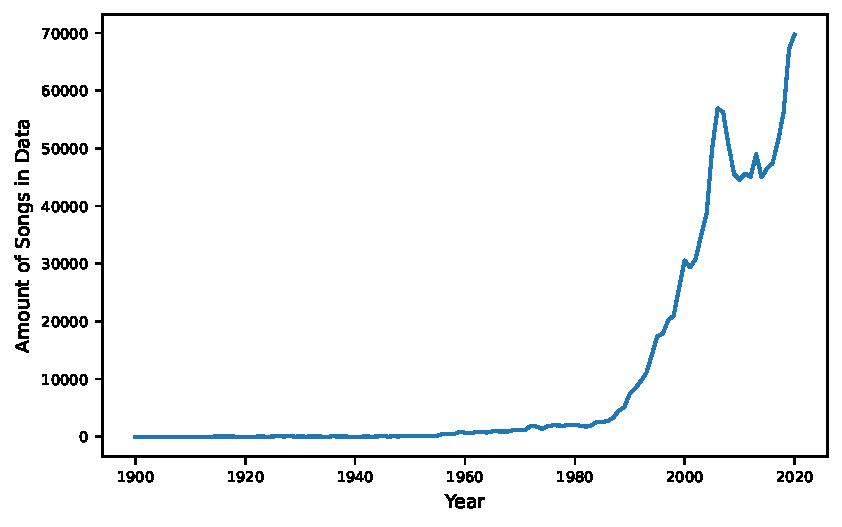
\includegraphics{data_spread}
  \caption{Some caption.}
\end{figure}

\section{Methodology}
This section will describe how the predictor was build and how this lead to the final result of the report.

\subsection{Preprocessing}

For validation of the predictor, the dataset was divided into a train- and a test-set, in a fairly standard 80-20 split. With that a validation of the resulting coefficients is possible.
To ensure comparable coefficients, the data was then centered to 0 and scaled to unit variance. 

Predicting the exact year, a song was released based on a number of features that roughly describe how it sounds is all but impossible. Additionally it is not that helpful in finding out which features are typical for a certain time period.
Therefore the labeling of the songs was not done by year, but by 5-year timespan. Fig 1b \answerTODO{} shows the number of samples in each of these timespans.

\subsection{Logistic Regression}

\answerTODO something about the sklearn Logistic regression process (MAP\dots)

The logistic regression process provides us with a number of coefficients, that tell us how prevalent the predictor estimated a certain feature in a given timespan. In other words, when the coefficient of timespan $A$ and feature $B$ is high, then feature $B$ is likely to be high for any song, placed in timespan $A$ by the predictor.


\section{Results}

\subsection{Predictor}

In order to evaluate our predictor, its prediction on the test set is compared to the results of assigning a timespan to each song completely at random.

\subsection{Coefficients}

\section{Conclusion}

Because we know very little about the dataset, these results do not really tell us that much. If for example, we knew, the dataset was made up of the most popular songs in each year, the resulting coefficients would be much more telling, as we could make statements about the development of \emph{popular} music over time. Because we know nothing of the sorts however, the dataset could be a completely random selection of songs or it could be extremely biased in ways that we cannot possibly predict. 

\bibliography{references} 

\end{document}
